\chapter{协议实现和性能分析}
\section {协议实现}
\subsection{协议流程}
%    \begin{algorithm}  
%    	\caption{Calculate $y = x^n$}   
%    	\label{alg1}  
%   	\begin{algorithmic} 	 
%    		\REQUIRE $n \geq 0 \vee x \neq 0$   
%    		\ENSURE $y = x^n$   
%    		\STATE $y \Leftarrow 1$   
%    		\IF{$n < 0$}   
%    		\STATE $X \Leftarrow 1 / x$   
%   		\STATE $N \Leftarrow -n$   
%    		\ELSE   
%    		\STATE $X \Leftarrow x$   
%    		\STATE $N \Leftarrow n$  
%    		\ENDIF   
%    		\WHILE{$N \neq 0$}   
%   		\IF{$N$ is even}   
%    		\STATE $X \Leftarrow X \times X$   
%    		\STATE $N \Leftarrow N / 2$   
%    		\ELSE[$N$ is odd]   
%    		\STATE $y \Leftarrow y \times X$   
%    		\STATE $N \Leftarrow N - 1$   
%    		\ENDIF   
%    		\ENDWHILE  
%    	\end{algorithmic}  
%    \end{algorithm}  

状态转移图
RXSTATE

 \begin{figure}[!ht]
 	\centering
 	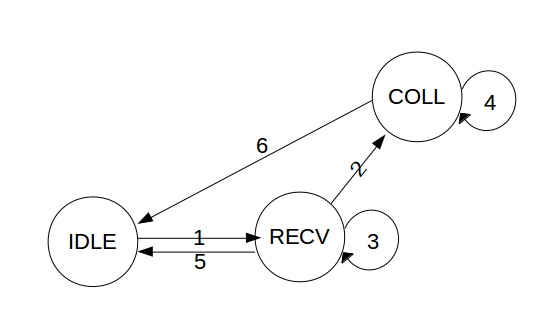
\includegraphics[scale=0.5]{figures/rxstate.png}
 	\caption{
 		rxstate
 	}
 	\label{fig:example}
 \end{figure}
 
\begin{table}[!ht]
	\centering
\begin{tabular}{c c c}
	\hline  % 在表格最上方绘制横线
	 &状态转移条件&执行的操作\\
	\hline  % 在表格最上方绘制横线
	1&节点空闲状态下侦听到包 & 接收包到pktRx\_\\
	2&节点接收状态下收到其他包,不满足接收条件&节点状态置为冲突状态,清空pktRx\_\\
	3&在接收状态下收到其他包,满足接收条件&节点设置NAV推迟接入,接收新包到pktRx\_,接收完毕后节点状态置为空闲\\
	4&在冲突状态下收到其他包,不满足接收条件&节点状态仍为冲突状态,清空pktRx\_\\
	5&在接收状态下接收完到达包以后&节点状态置为空闲\\	
	6&在冲突状态下收到其他包,满足接收条件&节点设置NAV推迟接入,接收新包到pktRx\_,接收完毕后节点状态置为空闲\\
	\hline
\end{tabular}
\end{table}

txstate
 \begin{figure}[!ht]
 	\centering
 	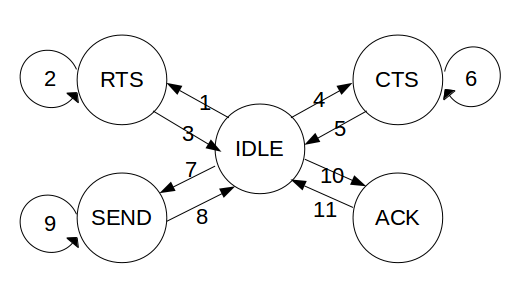
\includegraphics[scale=0.5]{figures/txstate.png}
 	\caption{
 		txstate
 	}
 	\label{fig:example}
 \end{figure}
 
\begin{table}[!ht]
	\centering
	\begin{tabular}{c c c}
		\hline  % 在表格最上方绘制横线
		&状态转移条件&执行的操作\\
		\hline  % 在表格最上方绘制横线
		1&节点准备开始一次数据传输 &准备pktRTS\_、pktTx\_,节点状态置为RTS\\
		2&RTS状态下接收到RTS、DATA、ACK、BCT包&节点状态不变,丢弃除BCT以外的接收到的包\\
		3&RTS状态下接收到CTS包清空pktRTS\_后或RTS状态超时&发送状态置为空闲,开始下一次发送\\
		4&接收完RTS包,发送状态空闲&准备pktCTRL\_,发送状态置为CTS,发送CTS包\\
		5&CTS状态下接收到DATA包清空pktCTRL\_后或CTS状态超时&发送状态置为空闲,开始下一次发送\\
		6&CTS状态下接收到RTS、CTS、ACK、BCT包&节点状态不变,丢弃除BCT以外的接收到的包\\
		7&接收完CTS包,发送状态空闲&准备pktTx\_发送状态置为MAC\_SEND,发送DATA包\\
		8&SEND状态下接收到ACK包清空pktTx\_后或SEND状态超时&发送状态置为空闲,开始下一次发送\\
		9&SEND状态下接收到RTS、CTS、DATA、BCT包&节点状态不变,丢弃除BCT以外的接收到的包\\
		10&接收完DATA包,发送状态空闲&准备pktCTRL\_,发送状态置为ACK,发送ACK包\\
		11&ACK发送完成&发送状态置为空闲,开始下一次发送\\
		\hline
	\end{tabular}
\end{table}

\subsection{帧格式}
BCT\\
\begin{tabular}{|c|c|c|}% 通过添加 | 来表示是否需要绘制竖线
	\hline  % 在表格最上方绘制横线
	名称&功能描述&字段位数(字节)\\
	\hline  %在第一行和第二行之间绘制横线
	Frame Control& &2\\
	\hline % 在表格最下方绘制横线
	Duration&持续时间&2\\
	\hline
	Receiver Address&接收节点地址&6\\
	\hline
	Transmitter Address&发送节点地址&6\\
	\hline
	网络负载情况&分为高低两种&1\\
	\hline
	Transmitter Address&发送节点地址&1\\
	\hline
	FCS&帧校验序列,用来检查所收到帧的完整性&4\\
	\hline
\end{tabular}

RTS/CTS/ACK\\
\begin{tabular}{|c|c|c|}% 通过添加 | 来表示是否需要绘制竖线
	\hline  % 在表格最上方绘制横线
	名称&功能描述&字段位数(字节)\\
	\hline  %在第一行和第二行之间绘制横线
	Frame Control&帧的subtype位,1011代表RTS,1100 CTS,1101 ACK&2\\
	\hline % 在表格最下方绘制横线
	Duration&持续时间&2\\
	\hline
	Receiver Address&接收节点地址&6\\
	\hline
	Transmitter Address&发送端地址,RTS帧的发送端的地址。&6\\
	\hline
	FCS&帧校验序列,用来检查所收到帧的完整性&4\\
	\hline
\end{tabular}

DATA\\
\begin{tabular}{|c|c|c|}% 通过添加 | 来表示是否需要绘制竖线
	\hline  % 在表格最上方绘制横线
	名称&功能描述&字段位数(字节)\\
	\hline  %在第一行和第二行之间绘制横线
	Frame Control&  &2\\
	\hline % 在表格最下方绘制横线
	持续时间(Duration ID)&用来记载网络分配矢量(Network Allocation Vector,简称NAV)&2\\
	\hline
	目的地址&最后的接收端,即负责将帧交付上层协议处理的工作站&6\\
	\hline
	源地址&传送的来源&6\\
	\hline
	接收端地址&负责处理该帧的无线工作站&6\\
	\hline
	顺序控制字段(Seq-Ctl)&用来重组帧片段以及丢弃重复帧&2\\	
	\hline
	发送端地址&将帧传送至无线媒介的无线接口&6\\
	\hline
	FCS&帧校验序列,用来检查所收到帧的完整性&4\\
	\hline
\end{tabular}

\section {性能分析}
按照流量模型,信道时间可以划分为信道繁忙时间和信道空闲时间,信道的平均利用率等于发送有效数据的时间和总时间的比值。
\begin{equation}
S=\frac{\overline U}{\overline O+\overline I}
\end{equation}

其中,$\overline U$表示发送有效数据传输时间的期望值,$\overline O$表示信道繁忙时间的期望值,$\overline I$表示信道空闲时间的期望值。
	
\subsection {低负载模式}
在MAPA-CSMA协议中,隐藏终端传输的RTS帧和移动节点定时发送的BCT帧会引起冲突。对于第一种情况,移动节点$\alpha$是固定节点$\omega$和固定节点$\beta$的邻居节点,节点$\beta$是节点$\omega$的隐藏终端。节点$\alpha$在和节点$\omega$进行数据交互的过程中,节点$\beta$发送的RTS帧可能会使得节点$\alpha$接收$\omega$的RTS帧和DATA帧产生碰撞。第二种情况中,除$\alpha$以外的其他邻居移动节点发送的BCT帧会对$\omega$接收CTS和ACK帧产生碰撞。

假设$P_S$是信道传输的成功概率,也就是在节点$\omega$数据交互周期内没有发生包碰撞的概率。节点$\omega$的邻居节点数量为M。$\omega$邻居移动节点的隐藏终端数量假设为Q,其中固定终端数量为$Q_s$,移动终端为$Q_m$,。任一隐藏终端以$\lambda/N$的速率向移动节点$\alpha$发送RTS包。移动节点$\alpha$以$\mu$的速率定时发送BCT包。

随机退避时间$CW_{min}=W$,$CW_{max}=2_r W$,在第i阶段的退避过程中可随机选择的退避时间为:
\begin{equation}
W_i=2^iW_i \ \ \ i\in(0,r)
\end{equation}
为了简化模型,只考虑第一阶段的退避过程,可选择的退避时间为$(0,W)$。

信道传输成功概率为:
\begin{equation}
P_S=\lambda(1-\lambda)^{M+Q_s}(1-\mu)^{Q_m}
\end{equation}

节点推迟接入包括接收到邻居节点的RTS帧和接收到邻居节点响应隐藏终端RTS帧而发送的CTS帧,因收到RTS帧推迟接入的概率为
\begin{equation}
 P_{Rdefer}=(1-\lambda)\lambda M
\end{equation}
因收到CTS帧推迟接入的概率为
\begin{equation}
 P_{Cdefer}=(1-\lambda)\lambda Q
\end{equation}

一个失败周期的持续时间是等待发送RTS帧的时间和发送RTS未收到CTS回复的超时时间,设最大传输时延为$\tau$
\begin{equation}
\begin{aligned}
T_{fail}&=T_{DIFS}+\overline W+Tout_{RTS}\\
&=T_{DIFS}+\overline W+T_{RTS}+2\tau+T_{SIFS}+T_{CTS}
\end{aligned}
\end{equation}

一个成功周期的持续时间包括了RTS,CTS,DATA和ACK的一整个流程。
\begin{equation}
T_{suc}=T_{DIFS}+\overline W+T_{RTS}+T_{CTS}+T_{DATA}+T_{ACK}+4\tau+3T_{SIFS}
\end{equation}

因收到RTS帧推迟接入的时间为
\begin{equation}
T_{Rdefer}=T_{CTS}+T_{DATA}+T_{ACK}+3\tau+3T_{SIFS}
\end{equation}

因收到CTS帧推迟接入的时间为
\begin{equation}
T_{Rdefer}=T_{DATA}+T_{ACK}+2\tau+2T_{SIFS}
\end{equation}

\begin{equation}
\overline B=T_{suc}P_S+T_{fail}(\lambda-P_S )+ T_{Cdefer}P_{Cdefer}+T_{Rdefer}P_{Rdefer}
\end{equation}

信道空闲时间为:
\begin{equation}
\overline I=\left\{
\begin{aligned}
1-B \ \ \ \ \ \ \ \ B<1\\
0\ \ \ \ \ \ \ \    B\ge 1
\end{aligned}
\right.
\end{equation}

根据吞吐量公式,计算得单一节点的吞吐量$(S)$为
\begin{equation}
\begin{aligned}
S&=\frac{\overline U}{\overline B+\overline I}\\&=\frac{T_{DATA}}{ T_{suc}P_S+T_{fail}(\lambda-P_S )+ T_{Cdefer}P_{Cdefer}+T_{Rdefer}P_{Rdefer}+\overline I}
\end{aligned}
\end{equation}

\subsection {高负载模式}

信道传输成功概率为:
\begin{equation}
P_S=\frac{\lambda}{2}(1-\frac{\lambda}{2})^{M+Q_s}(1-\mu)^{Q_m}
\end{equation}

节点推迟接入包括接收到邻居节点的RTS帧和接收到邻居节点响应隐藏终端RTS帧而发送的CTS帧,因收到RTS帧推迟接入的概率为
\begin{equation}
P_{Rdefer}=(1-\frac{\lambda}{2})\cdot\frac{\lambda}{2} M
\end{equation}
因收到CTS帧推迟接入的概率为
\begin{equation}
P_{Cdefer}=(1-\frac{\lambda}{2})\cdot\frac{\lambda}{2} Q
\end{equation}

一个失败周期的持续时间是等待发送RTS帧的时间和发送RTS未收到CTS回复的超时时间,设最大传输时延为$\tau$
\begin{equation}
\begin{aligned}
T_{fail}&=T_{DIFS}+\overline W+Tout_{RTS}\\
&=T_{DIFS}+\overline W+T_{RTS}+2\tau+T_{SIFS}+T_{CTS}
\end{aligned}
\end{equation}

一个成功周期的持续时间包括了RTS,CTS,2DATA和ACK的一整个流程。
\begin{equation}
T_{suc}=T_{DIFS}+\overline W+T_{RTS}+T_{CTS}+2T_{DATA}+T_{ACK}+4\tau+4T_{SIFS}
\end{equation}

因收到RTS帧推迟接入的时间为
\begin{equation}
T_{Rdefer}=T_{CTS}+2T_{DATA}+T_{ACK}+3\tau+4T_{SIFS}
\end{equation}

因收到CTS帧推迟接入的时间为
\begin{equation}
T_{Rdefer}=2T_{DATA}+T_{ACK}+2\tau+2T_{SIFS}
\end{equation}

信道繁忙时间为:
\begin{equation}
\overline B=T_{Cdefer}P_{Cdefer}+T_{Rdefer}P_{Rdefer}
\end{equation}

信道空闲时间为:
\begin{equation}
\overline I=\left\{
\begin{aligned}
1-B \ \ \ \ \ \ \ \ B<1\\
0\ \ \ \ \ \ \ \    B\ge 1
\end{aligned}
\right.
\end{equation}

根据吞吐量公式,计算得单一节点的吞吐量$(S)$为
\begin{equation}
\begin{aligned}
S&=\frac{\overline U}{\overline B+\overline I}\\&=\frac{2T_{DATA}}{ T_{suc}P_S+T_{fail}(\lambda-P_S )+ T_{Cdefer}P_{Cdefer}+T_{Rdefer}P_{Rdefer}+\overline I}
\end{aligned}
\end{equation}

\endinput